\documentclass[10pt]{article}
\usepackage{float}
\usepackage{amsmath}
\usepackage{listings}
\usepackage{graphicx}
\graphicspath{ {./images/} }
\begin{document}
{\centering
    CSU44061 Machine Learning - Week 3
    \par
    Samuel Petit - 17333946
    \par
    Dataset \# id:16-16-16
    \par
}
\section*{Question i}
Code for all questions provided in the appendix.
\subsection*{Part a}
Using code provided in the assignment, adding labels and titles,
I obtain the following graph, displaying the train data and their associated
output.


It seems that the data lies in a plane as it is quite flat.

\begin{center}
    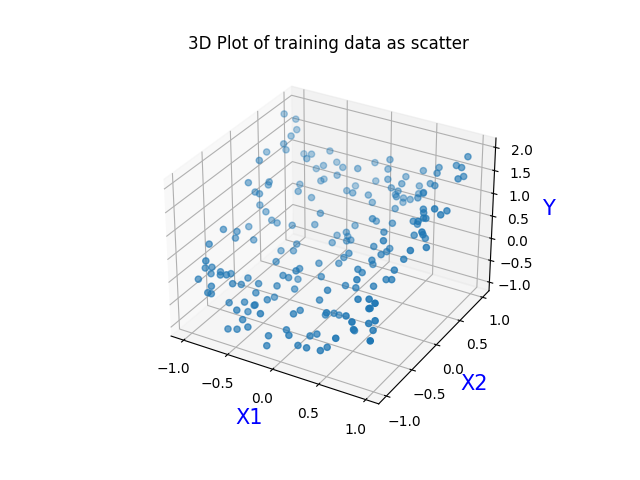
\includegraphics[scale=0.5]{Figure_1.png}
\end{center}


\subsection*{Part b}
As suggested, I used the PolynomialFeatures to create new features
going up to the power of 5 for both our available features $X_{1}$ and $X_{2}$.
Using these new features, we can train models. In this case, a Lasso model with
C values of 1, 200 and 5000. I chose these as they seemed to give me a range interesting
coefficients. Here are the parameters obtained from training a model with these 3 values for C:

\vspace{5mm} %5mm vertical space

C = 1
\par
Intercept: $0.3866779957293107$
\par
Coefficients:
\begin{equation*}
    [0, 0, 0, 0, -0, -0, 0, 0, 0, 0, 0, -0, 0, -0, -0, 0, 0, 0, 0, 0, 0]    
\end{equation*}

\vspace{5mm} %5mm vertical space

C = 200
\par
Intercept: $0.051955900546351685$
\par
Coefficients:
\begin{equation*}
    [ 0, -0.00314985, 0.96742042, 0.87629499, -0.00654177, 0.00630364, 
\end{equation*}
\begin{equation*}
    -0, 0, -0, 0, 0.06296949, -0, 0, -0, 0,-0, 0,-0, 0, -0, -0]    
\end{equation*}

\vspace{5mm} %5mm vertical space

C = 5000
\par
Intercept: $-0.00883716709265242$
\par
Coefficients:
\begin{equation*}
    [ 0, 0, 1.00631362, 0.88266399, -0.07027632, 0.23958815,
\end{equation*}
\begin{equation*}
    0.30758898, 0,-0.44969477, -0.0277997, 0.14749331, -0.00335293,
\end{equation*}
\begin{equation*}
    -0.10920998, 0.05252247, -0.15571219, -0.36071504, 0.19936564,
\end{equation*}
\begin{equation*}
    0.22193872, -0.22696517, 0.32680584, -0.]
\end{equation*}


We notice that as C gets bigger, more and more coefficients come into play.
For instance, using $C=1$ resulted in all coefficients being 0. A great value for C,
such as $C = 200$ results in a model where some coefficients are non-zero. In our case that is
6 coefficients. Finally, a very big value for C such as $C = 5000$ makes most of our models
parameters non-zero.

We can thus observe that a low value of C tends to set as many parameters as possible to 0.

I picked these C values so that I found resulting model parameters organised as such,
where we can clearly see the amount of non-zero parameters for each model.

  
\subsection*{Part c}
For this section, I reduced the grid range to [-1.3, 1.3]
since a bigger range made the predictions range too large for the y values, thus making it 
impossible to see the training data plane. I used the plot\_trisurf command
for plotting the training data as a surface. This yeilds the first plot (training data alone).
Then, adding the predictions to the plot we obtain the following 3 plots:

\begin{figure}[H]       
    \fbox{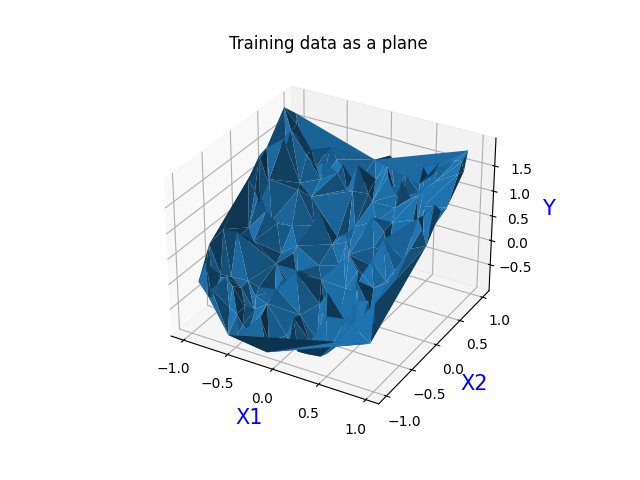
\includegraphics[scale=0.4]{Figure_2.png}}   
    \fbox{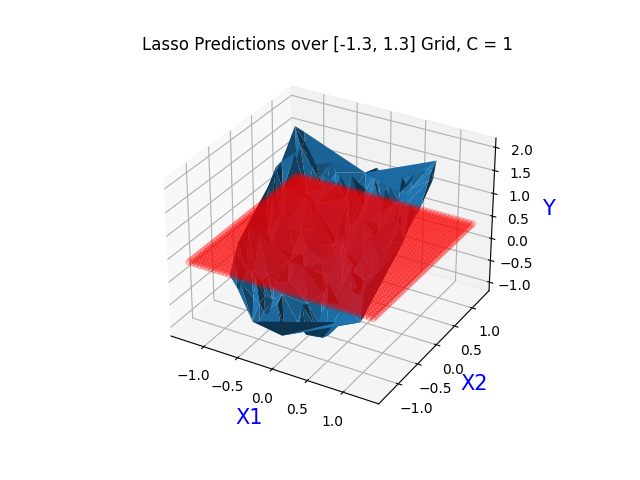
\includegraphics[scale=0.4]{Figure_3.png}}   
    \fbox{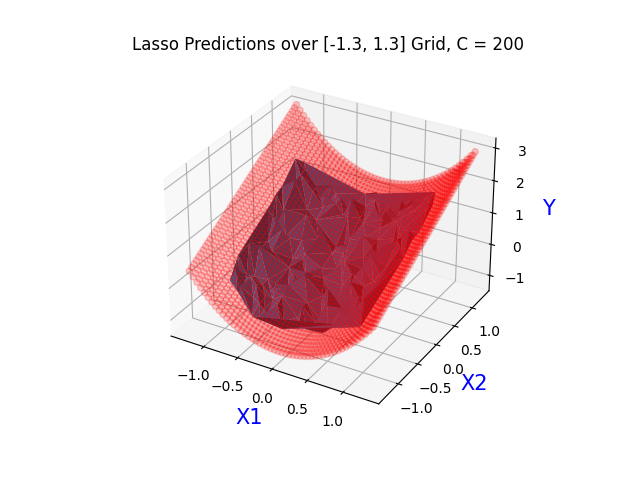
\includegraphics[scale=0.4]{Figure_4.png}}
    \fbox{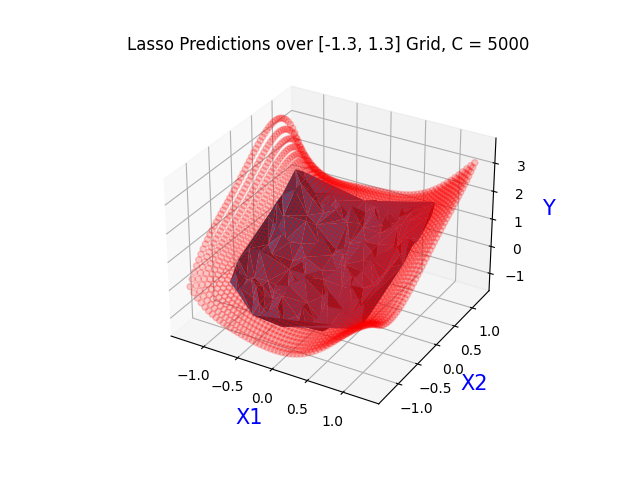
\includegraphics[scale=0.4]{Figure_5.png}}
\end{figure}

We notice that a value of $C = 1$ yeilds a flat plane, this is expected as all of the
models parameters are 0. Then, as we increase C and as more parameters come into play,
the predictions become more and more complex. We can also notice that the more
coefficents come into play, the more noise is taken into account by the model
predictions.


\subsection*{Part d}
Under-fitting is making a model so simple that it does not capture the
true complexity of a training data. For example trying to predict a
quadratic line using a linear model would be under-fitting as the predictions will
be quite poor.

Over-fitting is the opposite. That is using too many features such that the model
matches training data too closely and thus matches more noise that we likely do not want.

Taking this knowledge and comparing it to our models and plots above, we notice the following:

- The model with C = 1 is an example of underfitting. All of our coefficients are 0 thus
none of the feature values are used to make predictions, our plot is a simple plane 
and we notice that it does not match accurately our training data.

- The model with C = 5000 is an example of over-fitting, we notice that all or almost all 
coefficients are used by the model thus making using of many features which may 
or may not be useful for predictions. Looking at the plot we notice how it is much more complex
and fits noise from our training data with the many ups and downs that are noticeable on the predictions.


\subsection*{Part e}
Similarly, I used the PolynomialFeatures to create the same features as with the previous questions up
to a power of 5.

Training a Ridge regression model using the following C values: 0.00001, 1, 200 yeilds the following
model parameters:

\vspace{5mm} %5mm vertical space

C = 0.00001
\par
Intercept: $0.38649423514736153$
\par
Coefficients:
\begin{equation*}
    [ 0.00000000e+00, 1.51458548e-04, 1.47029680e-03, 3.40428762e-04
\end{equation*}
\begin{equation*}
    -4.46143189e-05, -9.72722585e-06, 6.50007693e-05, 5.18327561e-04
\end{equation*}
\begin{equation*}
    1.43993794e-04, 9.12639486e-04, 3.19489175e-04, -2.50299601e-05
\end{equation*}
\begin{equation*}
    9.40108739e-05, -2.14996644e-05, -1.26054105e-05, 3.83327579e-05
\end{equation*}
\begin{equation*}
    3.23922402e-04, 6.38460692e-05, 3.09930239e-04, 1.35033294e-04
\end{equation*}
\begin{equation*}
    6.60283127e-04]
\end{equation*}

\vspace{5mm} %5mm vertical space

C = 1
\par
Intercept: $0.02671319631416863$
\par
Coefficients:
\begin{equation*}
    [0, 0.00897235, 0.93984335, 0.70409046, -0.05097339, 0.16709087
\end{equation*}
\begin{equation*}
    0.1100758, 0.09688451, -0.19635685, 0.07396169, 0.30812562, -0.04912464
\end{equation*}
\begin{equation*}
    -0.02268318, 0.05130517, -0.108326, -0.14242707, 0.06966072, 0.12227828
\end{equation*}
\begin{equation*}
    -0.16703029, 0.08436703, -0.04872375]
\end{equation*}

\vspace{5mm} %5mm vertical space

C = 200
\par
Intercept: $-0.02759728211480622$
\par
Coefficients:
\begin{equation*}
    [ 0, -0.00662543, 0.99248296, 0.89984203, -0.14267824, 0.3603547
\end{equation*}
\begin{equation*}
    0.57425937, 0.07124828, -0.79767503, 0.00522424, 0.1531058, 0.01859584
\end{equation*}
\begin{equation*}
    -0.20079551, 0.17207762, -0.2688553, -0.65605953, 0.27619337, 0.37207688
\end{equation*}
\begin{equation*}
    -0.45549789, 0.64632594, -0.00373098]
\end{equation*}


For this regression model, we notice that all coefficients are used for all values of C. However we also
notice that when C tends to 0 so do the coefficients, on the opposite, the higher value for C the less impact
the ridge term will have on its coefficients and thus that is why we only notice minor differences between C = 1 and C = 200.

I picked these C values so that we could observe the impact of a very small vs large C value thus 
displaying the impact of the ridge term on the Ridge regression.

  
For this section, I used the same grid range as in the previous question ([-1.3, 1.3]) such that it is easily visible and
y values don't go into a range to large.
since a bigger range made the predictions range too large for the y values, thus making it 
impossible to see the training data plane. I used the plot\_trisurf command
for plotting the training data as a surface. This yeilds the first plot (training data alone).
Then, adding the predictions to the plot we obtain the following 3 plots:

\begin{figure}[H]       
    \fbox{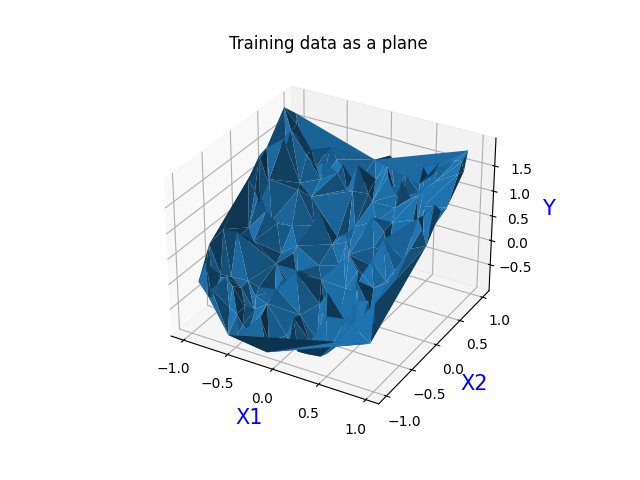
\includegraphics[scale=0.4]{Figure_2.png}}   
    \fbox{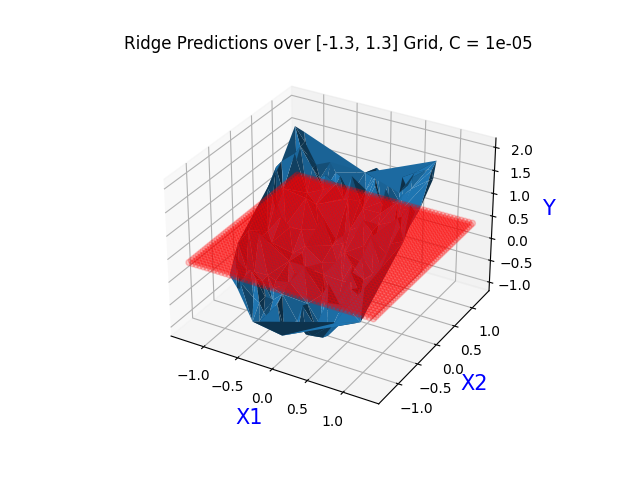
\includegraphics[scale=0.4]{Figure_6.png}}   
    \fbox{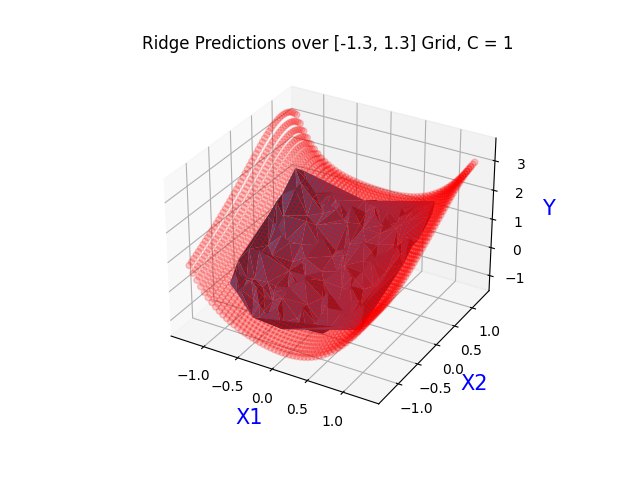
\includegraphics[scale=0.4]{Figure_7.png}}
    \fbox{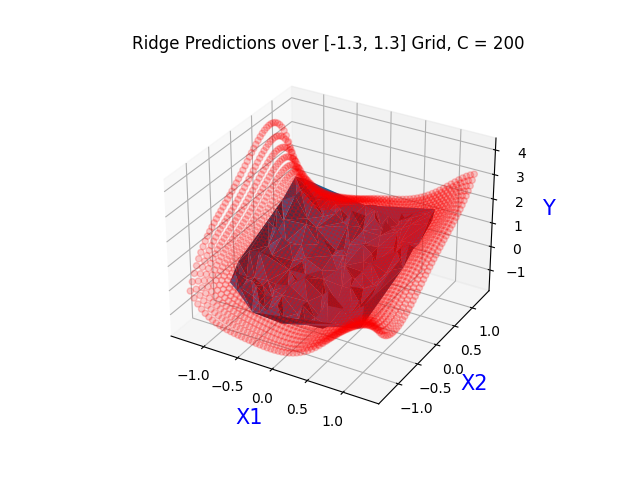
\includegraphics[scale=0.4]{Figure_8.png}}
\end{figure}

We notice that a value of $C = 0.00001$ yeilds a flat plane, this is expected given all of the
models parameters tend towards 0 as previously explained, this models is an example of underfitting. Then, as we increase C,
the model takes the ridge term less and less into account, the more our model fits our data and goes into overfitting.

\section*{Question ii}
\subsection*{Part a}

Using the provided fold values, we train a Lasso model for each of the folds,
for each model we compute the mean square error (using sklearn's "mean\_squared\_error" method).
Then, for each fold we compute the variance and mean of the mean squarred error.

Executing this for all of the folds we then obtain a variance and mean for each computed fold, thus
we can obtain the following plot:

\begin{center}
    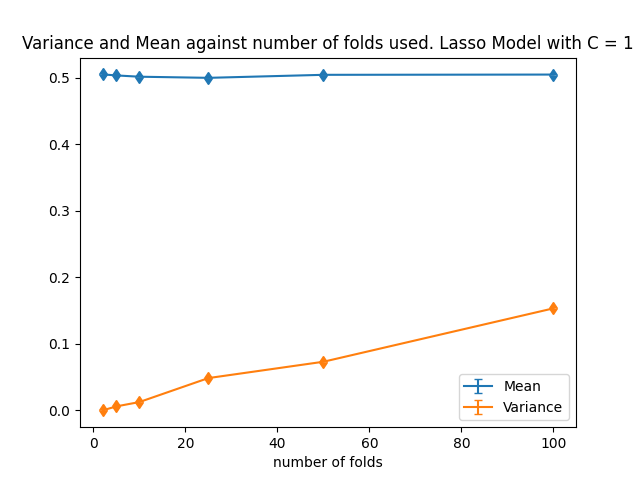
\includegraphics[scale=0.4]{Figure_9.png}
\end{center}


First of all, we notice that the mean is quite flat. That is to be expected. Remember from the previous question,
a lasso model with C = 1 yeilds a flat plane (ie all of its parameters are 0).
Let's look at the variance, we notice that as the number of folds increases, so does the variance.
That is to be expected given that our model is a baseline (constant model). Given that our dataset is quite small
(200 entries or so), picking a k too large (such as 100) will make for a very low number of testing values for each 
fold thus making the variance bigger.

In this case, given the size of our dataset and taking into account that we do not want too big of a variance,
picking k = 5 or k = 10 seem to be appropriate choices.

\subsection*{Part b}
I decided to pick k = 10. We execute the same steps as with the previous question, only this 
time changing the value of C and keeping a constant number of folds.
I decided to use a range of values for C going between 0.01 to 75 with a step size of 5.
This is because these values seemed to give the section of variation we are interested in,
making C go over 75 would give mostly the same values and similarly for going below 0.001.

We obtain the following plot:

\begin{center}
    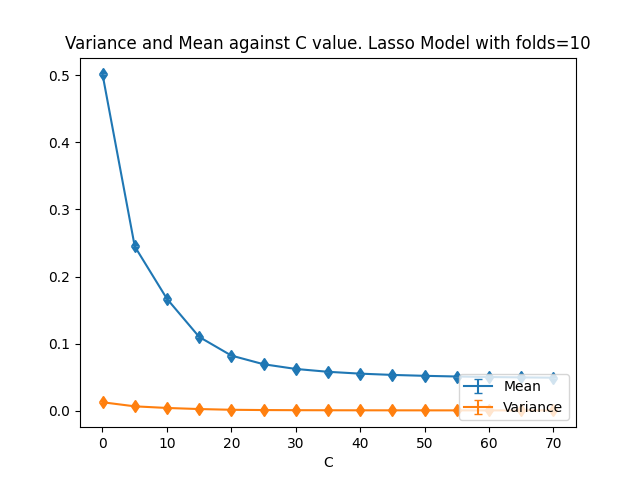
\includegraphics[scale=0.4]{Figure_10.png}
\end{center}

\subsection*{Part c}
Using the plot we obtain in part b, we notice that a low value for C (such as C = 1)
yeilds a mean of 0.5 which is very high, for such scenarios when C is very low, 
we have all coefficients set to 0 which explains we obtain such a high mean value.
On the opposite when C is too high, we essentially have a linear regression.

In this case it seems like the sweet spot is at C = 45 as it seems the be where the
mean squared error is stabilising.


\subsection*{Part d}
Using the same values and justification as with part b of this question,
we obtain the following plot:

\begin{center}
    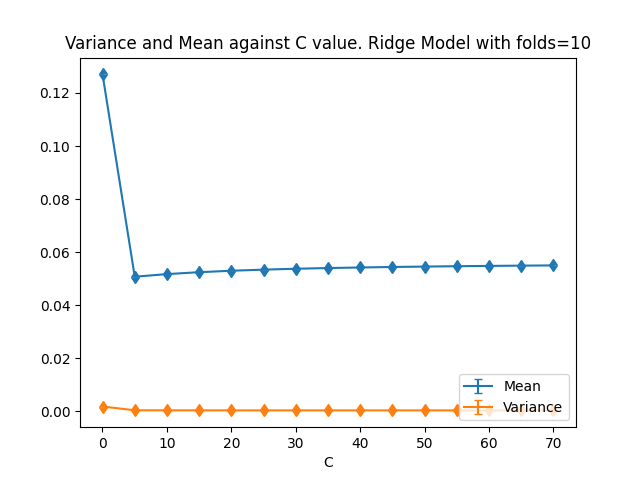
\includegraphics[scale=0.4]{Figure_11.png}
\end{center}

We notice that a low value for C (such as C = 1)
yeilds a mean of 0.12 which is the highest on this plot, for such scenarios when C is very low, 
we have all coefficients close to 0 which explains we obtain such a high mean value.
On the opposite when C is too high, the ridge term is essentially not taken into account.

In this case it seems like the sweet spot is at C = 5 as it seems the be where the
mean squared error is stabilising (and the lowest)



\section*{Appendix}
Question 1
\begin{lstlisting}
from sklearn.linear_model import Ridge
import matplotlib.pyplot as plt
import numpy as np
import pandas as pd
from sklearn.preprocessing import PolynomialFeatures
from sklearn import linear_model

# Read in data
df = pd.read_csv("week3.csv", comment='#')
X1 = df.iloc[:, 0]
X2 = df.iloc[:, 1]
X = np.column_stack((X1, X2))
y = np.array(df.iloc[:, 2])

# Plot Q1 a - 3D figure.
fig = plt.figure()
ax = fig.add_subplot(111, projection='3d')
ax.scatter(X[:, 0], X[:, 1], y)
ax.set_xlabel('X1', color='blue', size=15)
ax.set_ylabel('X2', color='blue', size=15)
ax.set_zlabel('Y', color='blue', size=15)
ax.set_title("3D Plot of training data as scatter")

# Q1 b training lasso models
# Grab the powers up to 5.
poly = PolynomialFeatures(5)
X_poly = poly.fit_transform(X)
# Generate the [-5,5] grid for predictions.
Xtest = []
grid = np.linspace(-1.3, 1.3)
for i in grid:
    for j in grid:
        Xtest.append([i, j])
# Grab the powers up to 5 for the grid data.
Xtest = np.array(Xtest)
Xtest_poly = poly.fit_transform(Xtest)

# Plot the plan with training data alone
fig = plt.figure()
ax = fig.add_subplot(111, projection='3d')
ax.plot_trisurf(X[:, 0], X[:, 1], y)
ax.set_xlabel('X1', color='blue', size=15)
ax.set_ylabel('X2', color='blue', size=15)
ax.set_zlabel('Y', color='blue', size=15)
ax.set_title("Training data as a plane")

# Question 1 b and c - using C = 1 200 and 500
for C in [1, 200, 5000]:
    # Note that alpha = 1 / C
    model = linear_model.Lasso(alpha=(1/C))
    model.fit(X_poly, y)
    ypred = model.predict(Xtest_poly)
    # Print model parameters
    print("c = ", C)
    print(model.intercept_)
    print(model.coef_)
    # Plot model predictions.
    fig = plt.figure()
    ax = fig.add_subplot(111, projection='3d')
    ax.scatter(Xtest[:, 0], Xtest[:, 1], ypred,
                        color="red", alpha=0.2)
    ax.plot_trisurf(X[:, 0], X[:, 1], y)
    ax.set_xlabel('X1', color='blue', size=15)
    ax.set_ylabel('X2', color='blue', size=15)
    ax.set_zlabel('Y', color='blue', size=15)
    ax.set_title("Lasso Predictions over " +
                "[-1.3, 1.3] Grid, C = " + str(C))

# Question e - Ridge Model
for C in [0.00001, 1, 200]:
    # Note that alpha = 1 / 2C for Ridge regression
    model = Ridge(alpha=(1/(2 * C)))
    model.fit(X_poly, y)
    ypred = model.predict(Xtest_poly)
    # Print model parameters.
    print("c = ", C)
    print(model.intercept_)
    print(model.coef_)
    # Plot model predictions.
    fig = plt.figure()
    ax = fig.add_subplot(111, projection='3d')
    ax.scatter(Xtest[:, 0], Xtest[:, 1],
            ypred, color="red", alpha=0.2)
    ax.plot_trisurf(X[:, 0], X[:, 1], y)
    ax.set_xlabel('X1', color='blue', size=15)
    ax.set_ylabel('X2', color='blue', size=15)
    ax.set_zlabel('Y', color='blue', size=15)
    ax.set_title("Ridge Predictions over " +
            "[-1.3, 1.3] Grid, C = " + str(C))
plt.show()
\end{lstlisting}

Question 2
\begin{lstlisting}
from sklearn.metrics import mean_squared_error
from sklearn.preprocessing import PolynomialFeatures
from sklearn.model_selection import KFold
from sklearn.linear_model import Ridge, Lasso
import numpy as np
import pandas as pd
import matplotlib.pyplot as plt
import statistics

# Read in data
df = pd.read_csv("week3.csv", comment='#')
X1 = df.iloc[:, 0]
X2 = df.iloc[:, 1]
X = np.column_stack((X1, X2))
y = np.array(df.iloc[:, 2])

# Get polynomials for features
poly = PolynomialFeatures(5)
X_poly = poly.fit_transform(X)

# Question a
# For each fold, keep track of means, variances and folds
means = []
variances = []
C = 1
all_folds = [2, 5, 10, 25, 50, 100]
for f in all_folds:
    # Split the dataset into folds
    kf = KFold(n_splits=f)
    mse = []
    # Train a model using each fold
    for train, test in kf.split(X_poly):
        model = Lasso(alpha=(1/C))
        model.fit(X_poly[train], y[train])
        ypred = model.predict(X_poly[test])
        # Keep the MSE for each model
        mse.append(mean_squared_error(y[test], ypred))
    # Store the mean, variance for each model
    means.append(statistics.mean(mse))
    variances.append(statistics.variance(mse))

# Plot the means and variances
fig = plt.figure()
ax = fig.add_subplot(111)
ax.errorbar(all_folds, means, label='Mean',
            yerr=all_folds, uplims=True, lolims=True)
ax.errorbar(all_folds, variances, label='Variance',
            yerr=all_folds, uplims=True, lolims=True)
ax.set_xlabel("number of folds")
ax.set_title(
    "Variance and Mean against number of folds used." +
    "Lasso Model with C = 1")
ax.legend(loc='lower right')

# Question b - Lasso model using 10-fold
means = []
variances = []
num_folds = 10
# Using a range of Cs between 1 and 75
# with a 5 increment per step.
C_range = np.arange(0.01, 75, 5)
for C in C_range:
    # Split the dataset in 10 folds
    kf = KFold(n_splits=num_folds)
    mse = []
    # Train a model for each fold
    for train, test in kf.split(X_poly):
        model = Lasso(alpha=(1/C))
        model.fit(X_poly[train], y[train])
        ypred = model.predict(X_poly[test])
        # Keep the MSE for each model
        mse.append(mean_squared_error(y[test], ypred))
    # Store all models folds variances and means.
    means.append(statistics.mean(mse))
    variances.append(statistics.variance(mse))

# Plot the means and variances
fig = plt.figure()
ax = fig.add_subplot(111)
ax.errorbar(C_range, means, label='Mean',
            yerr=C_range, uplims=True, lolims=True)
ax.errorbar(C_range, variances, label='Variance',
            yerr=C_range, uplims=True, lolims=True)
ax.set_xlabel("mean/variance")
ax.set_xlabel("C")
ax.set_title(
    "Variance and Mean against C value." +
    "Lasso Model with folds=10")
ax.legend(loc='lower right')

# Question d - Ridge model using 10 folds.
means = []
variances = []
num_folds = 10
for C in C_range:
    # Split the dataset in 10 folds
    kf = KFold(n_splits=num_folds)
    mse = []
    # Train a model for each fold
    for train, test in kf.split(X_poly):
        model = Ridge(alpha=(1/(2 * C)))
        model.fit(X_poly[train], y[train])
        ypred = model.predict(X_poly[test])
        # Keep the MSE for each model
        mse.append(mean_squared_error(y[test], ypred))
    # Store all models folds variances and means.
    means.append(statistics.mean(mse))
    variances.append(statistics.variance(mse))

# Plot the means and variances
fig = plt.figure()
ax = fig.add_subplot(111)
ax.errorbar(C_range, means, label='Mean',
            yerr=C_range, uplims=True, lolims=True)
ax.errorbar(C_range, variances, label='Variance',
            yerr=C_range, uplims=True, lolims=True)
ax.set_xlabel("mean/variance")
ax.set_xlabel("C")
ax.set_title(
    "Variance and Mean against C value." +
    "Ridge Model with folds=10")
ax.legend(loc='lower right')
plt.show()
\end{lstlisting}
\end{document}
